\section{Experimental Results}

% \begin{frame}<beamer>
% \frametitle{Outline}
% \tableofcontents[currentsection,currentsubsection]
% \end{frame}
\subsection*{Experiment Design}
\begin{frame}
\frametitle{Experiment Design}
\begin{itemize}
  \item We have fully implemented \WFD, \WFDINC, \WFDIP and \FFD 
  \item We compare all algorithms with a State-of-the-Art algorithm\footnote{We
  thank Kai M. Wurm and Wolfram Burgard for providing us their own
  implementation}
  \item Our system is based on \emph{GMapping} SLAM implementation
  	\begin{itemize}
  		\item \citep{grisetti05icra,grisetti07tro} 
  	\end{itemize} 
  \item Two machines: 
  	\begin{itemize}
  		\item Intel Core 2 Duo T6600 CPU, 2.20GHz, 4GB RAM
  		\item Intel Pentium III Coppermine CPU, 800MHz, 1GB RAM % not going to talk
  		% d about former results
  	\end{itemize} 
  \item We measured CPU-process time 
\end{itemize}
\end{frame}

\begin{frame}
\frametitle{Experiment Design}
\begin{itemize}
  \item All detection algorithms are executed when a map update occurs 
  \item \FFD is executed when a new laser reading is received 
  \item We accumulate \FFD's time between two map updates
  %calls to other algorithms
  \item Tested on data obtained from RADISH \citep{Radish}
  	\begin{itemize}
  	  \item Gold standard robotics dataset
  	  \item Provides exploration data obtained by \emph{real-world} robots
  	  %\item Gold standard of exploration community
  	  \item Tested on all maps contain exploration range readings data  
  	\end{itemize}  
\end{itemize}
\end{frame}


% \begin{frame}
% \frametitle{Experiment Design}
% \transdissolve
% 	\begin{figure}
% 	 \centering
% 	 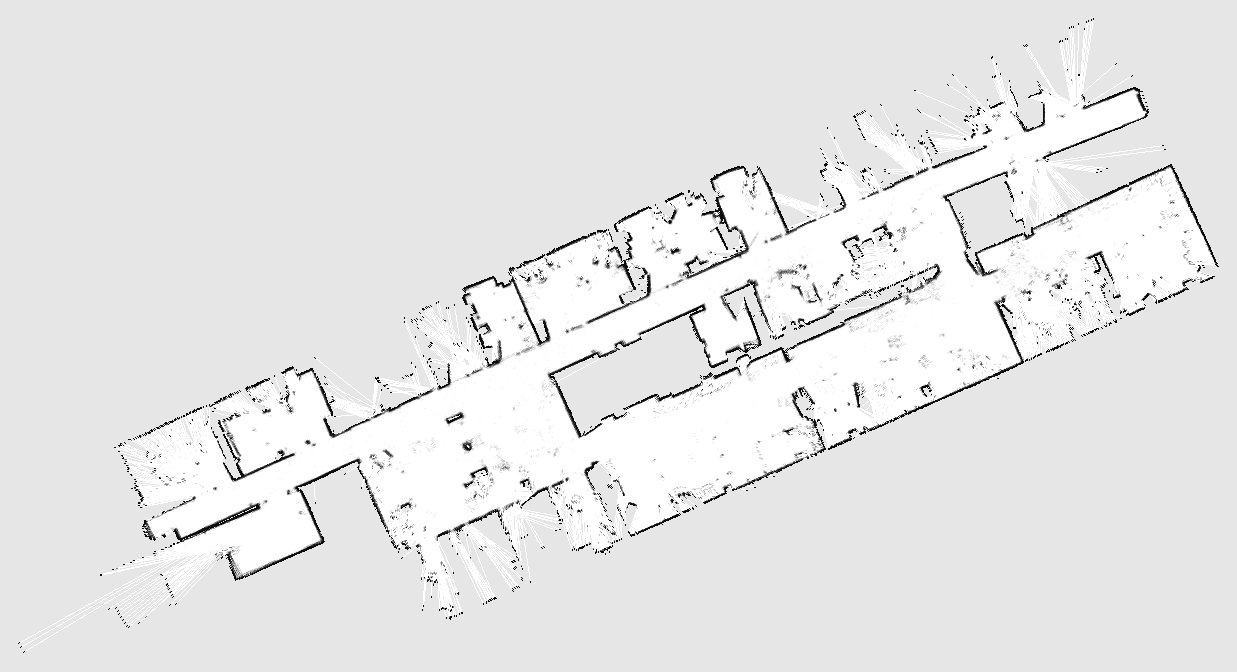
\includegraphics[width=0.85\columnwidth,keepaspectratio]{images/cartesium.JPG}
% 	\end{figure}
% \end{frame}


\begin{frame}
\frametitle{Experiment Design}
\transfade%\transdissolve
	\begin{figure}
	 \centering
	 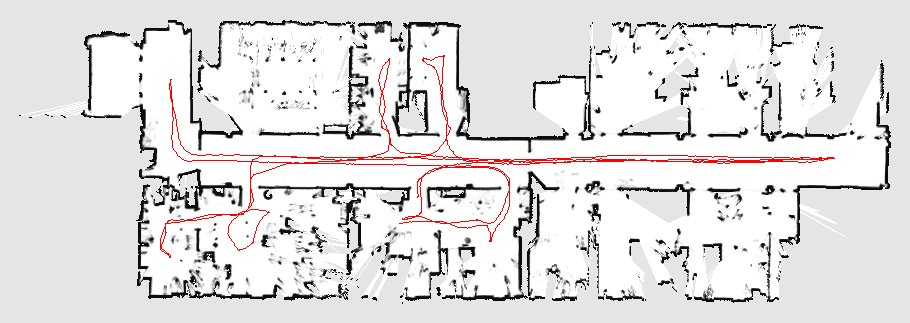
\includegraphics[width=1.05\columnwidth,keepaspectratio]{images/freiburg.JPG}
	 \caption{Example of a testing environment, University of Freiburg.  Image
	 was taken from RADISH, \cite{Radish}}
	\end{figure}
\end{frame}

\subsection*{Runtime Comparision}
\begin{frame}
\frametitle<1>{Runtime Comparision (Core 2 Duo)}
\frametitle<2>{Runtime Comparision (Coppermine)}
\transfade%\transdissolve
\pgfbox[center,center]{ 
        \begin{tikzpicture}[overlay,line width = 0.1cm, blue] 
		\node[color=blue,anchor=east, rotate=90] at (0.7,-1.3) (arrow_label) {better};
          \draw[->] (1,0) -- (1,-4); 
        \end{tikzpicture} 
      }
	\vspace{-10pt}
	\begin{figure}
	 \centering
	 %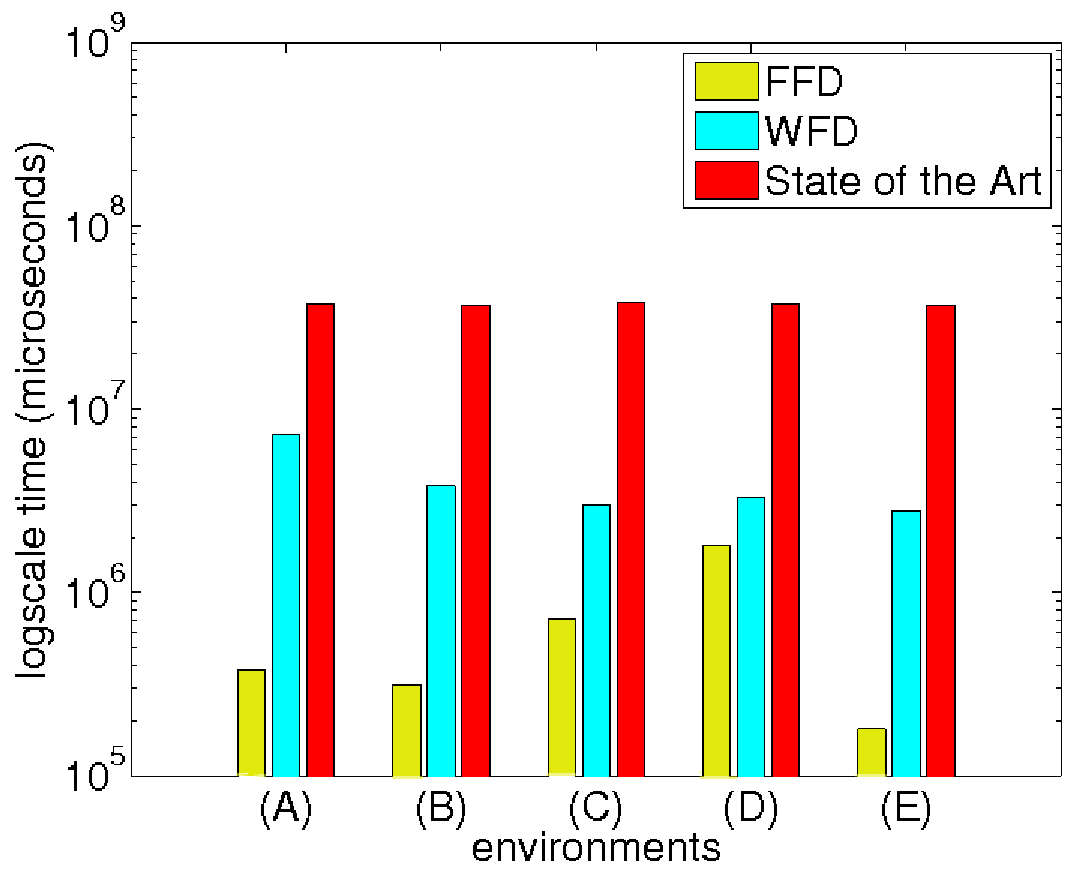
\includegraphics[width=0.65\columnwidth,keepaspectratio]{images/graph_Results_core2_yellow.pdf}
	 \includegraphics<1>[width=0.7\textwidth,keepaspectratio,angle=0]{../Thesis/graphs/plot_Results_five_algorithms.pdf}
	 \includegraphics<2>[width=0.7\textwidth,keepaspectratio,angle=0]{../Thesis/graphs/plot_Results_coppermine.pdf}
	\end{figure}
	\vspace{-10pt}
	\begin{itemize} 
  \item Y axis: mean execution time (microseconds) on a \emph{logaritmic scale} 
  \item \WFD,\WFDINC: faster than \SOTA by an order of magnitude 
  \item \FFD,\WFDIP: faster than \SOTA by two orders of magnitude 
\end{itemize}
\end{frame}

\begin{frame}
\frametitle{What Happend in Environment (D)?}

\begin{alertblock}{What Happend?}
	The mean run-time of \WFD is not relatively slower than \FFD
\end{alertblock}
\pause
\begin{exampleblock}{Answer}
	\begin{itemize}
	  \item Environment (D) contains regions that contains small obstacles
	  \item The obstacles enlarge the length of contour scanned by \FFD
	  \item As shown, the contour length affects the run-time complexity
	\end{itemize}
\end{exampleblock}

\begin{figure} 
 \centering
 \visible<2>{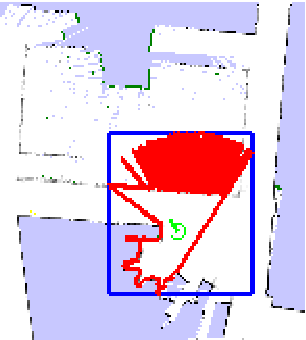
\includegraphics[width=0.25\columnwidth,keepaspectratio,angle=0]
 {../Thesis/images/environment_D_bad_contour_example2.pdf}}
\end{figure}

\end{frame}

\begin{frame}
\frametitle{Why is \WFDINC Sometimes Worse than \WFD?}

\begin{alertblock}{What Happend?}
	\begin{itemize}
	  \item In the worst-case, \WFDINC should perform the same as \WFD
		%\begin{itemize}
		%  \item Including an overhead of maintenance
		%\end{itemize}
	  \item The run-time means of \WFD and \WFDINC do not have a trend
	\end{itemize}
\end{alertblock}
\pause
\begin{exampleblock}{Hypothesis}
	\begin{itemize}
	  \item Certain environments have high frequency of particle
	  change
	  \item $\Rightarrow$ \WFDINC cleans its previous detected frontiers more often
	  
	\end{itemize}
\end{exampleblock}

\begin{table}
\centering
\begin{tabular}{|c|c|c||c|}
\hline \textbf{Map}&\textbf{Changes}&\textbf{Executions}&\textbf{Percent (\%)}
\\
\hline 
\hline (A)& 56 & 110 & 50.91  \\
\hline (B)& 52 & 287 & 18.12  \\
\hline (C)& 25 & 160 & 15.62  \\
\hline (D)& 193 & 429 & 44.99 \\ 
\hline (E)& 73 & 340 & 21.47 \\ \hline
\end{tabular}
\end{table}

\end{frame}

% \begin{frame}
% \frametitle{What Happend to \WFDIP in Environments (A),(C),(E), Weak Machine?}
% \begin{itemize}
%   \item Strong machine: \WFDIP outperforms all other algorithms
%   \item Weak machine: the situation is different in maps (A),(C),(E) \pause
%   \item Hypothesis (1) Memory: 
% 		\begin{itemize}
% 		  \item Weak machine is equipped with less RAM than strong machine
% 		  \item \WFDIP holds a separate instance of \WFDINC for each particle 
% 		  \item Hypothesis: strong machine runs each thread on a separate core
% 		  \item In our experiment, 30 instances of \WFDINC
% 		\end{itemize} \pause
%   \item Hypothesis (2) CPU: 
% 		\begin{itemize}
% 		  \item Weak machine is equipped a single CPU
% 		  \item GMapping runs two threads (Main thread and SLAM thread)
% 		  \item Hypothesis: strong machine runs each thread on a separate core  
% 		\end{itemize} 
% \end{itemize}
% \end{frame}

\subsection*{Evaluating FFD in a Finer Resolution}
\begin{frame}
\frametitle{Measuring Run-Time for Individual Particle}
\only<1>{
\begin{itemize}
  \item Particle-filter: each hypothesis runs its own instance of \FFD
  \item Investigate \FFD in a finer resolution
  \item Compare run-time of individual particles in each map
  %\item Each bar represents a specific particle
  %\item Vertical axis: measures the run-time of \FFD for the particle
  %\item Error-bars: the standard deviation of each particle's run-time
  
\end{itemize}
}
\only<2>{

\begin{figure}[htp]
%\vspace{-60pt}
 \centering 
 \subfigure[] {
 \centering
 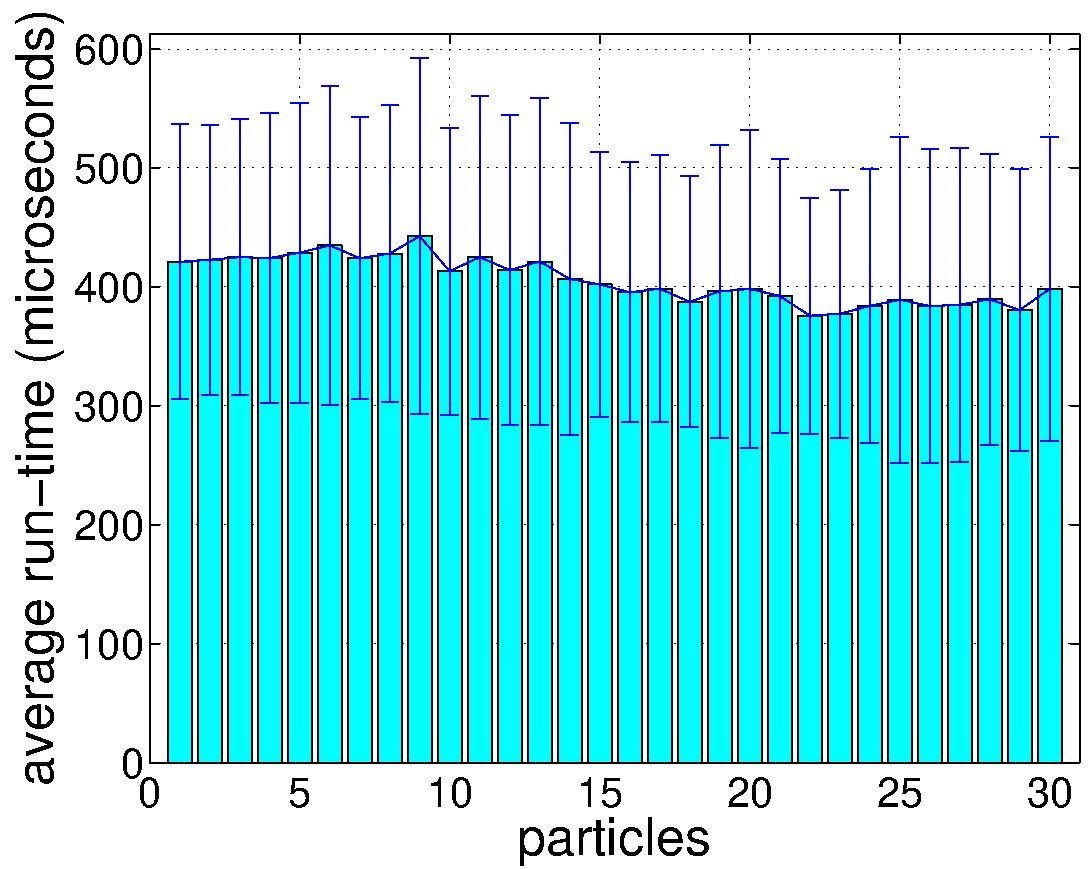
\includegraphics[width=0.31\columnwidth,keepaspectratio]{../Thesis/graphs/graph_particle_times_ubremen-cartesium-demo2.pdf}
 }
 \subfigure[] {
 \centering
 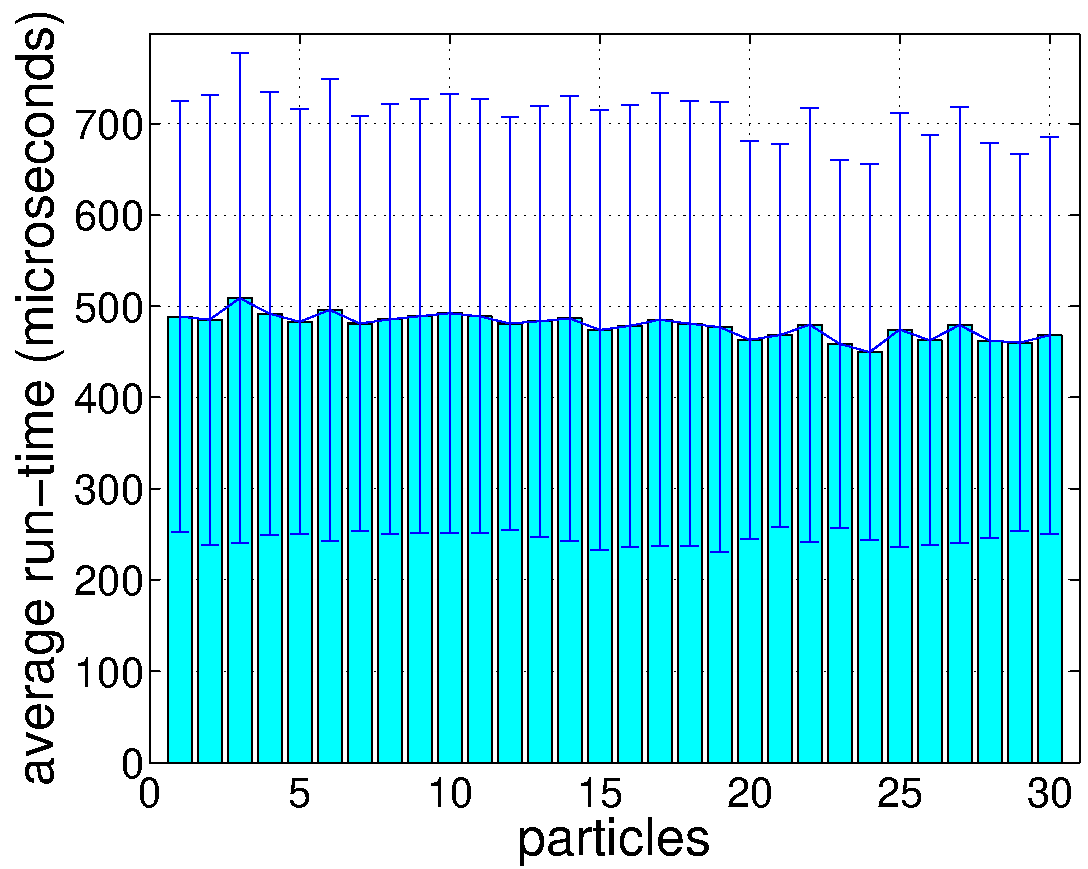
\includegraphics[width=0.31\columnwidth,keepaspectratio]{../Thesis/graphs/graph_particle_times_fr079-sm.pdf}
 }
 \subfigure[] {
 \centering
 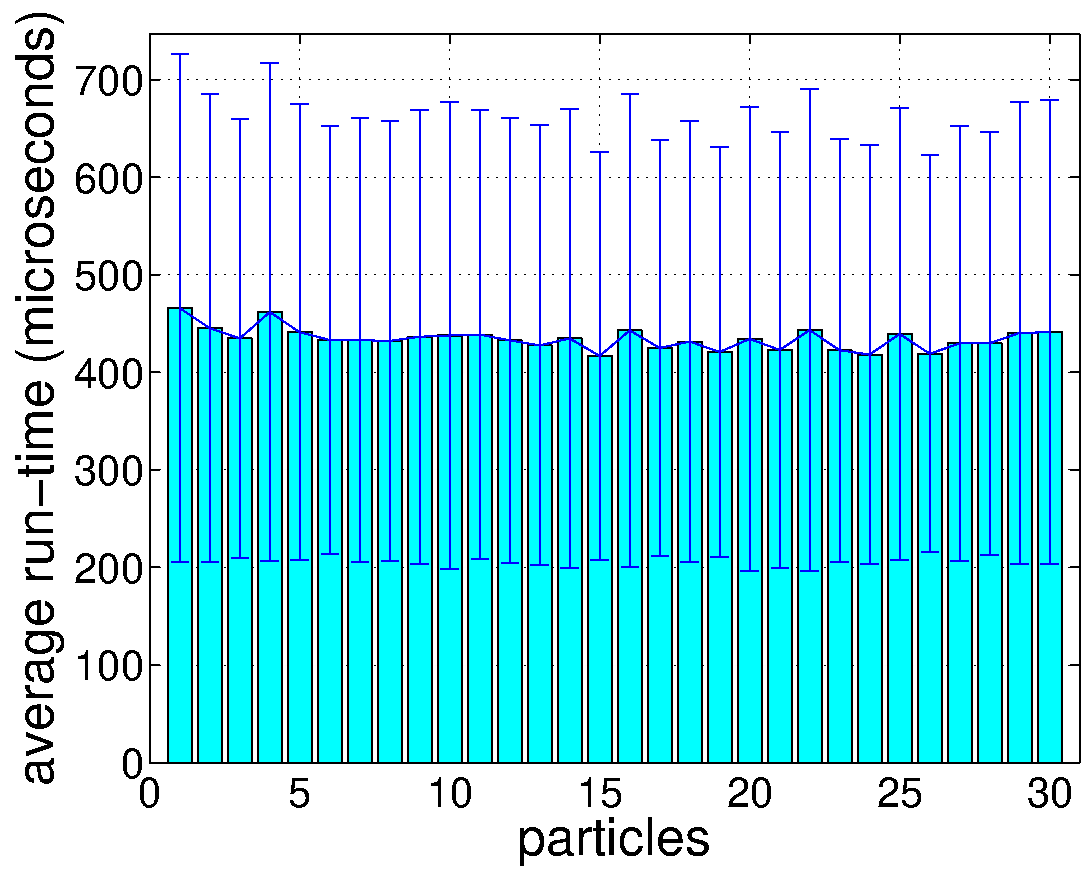
\includegraphics[width=0.31\columnwidth,keepaspectratio]{../Thesis/graphs/graph_particle_times_fr-campus-20040714.pdf}
 }
 \subfigure[] {
 \centering
 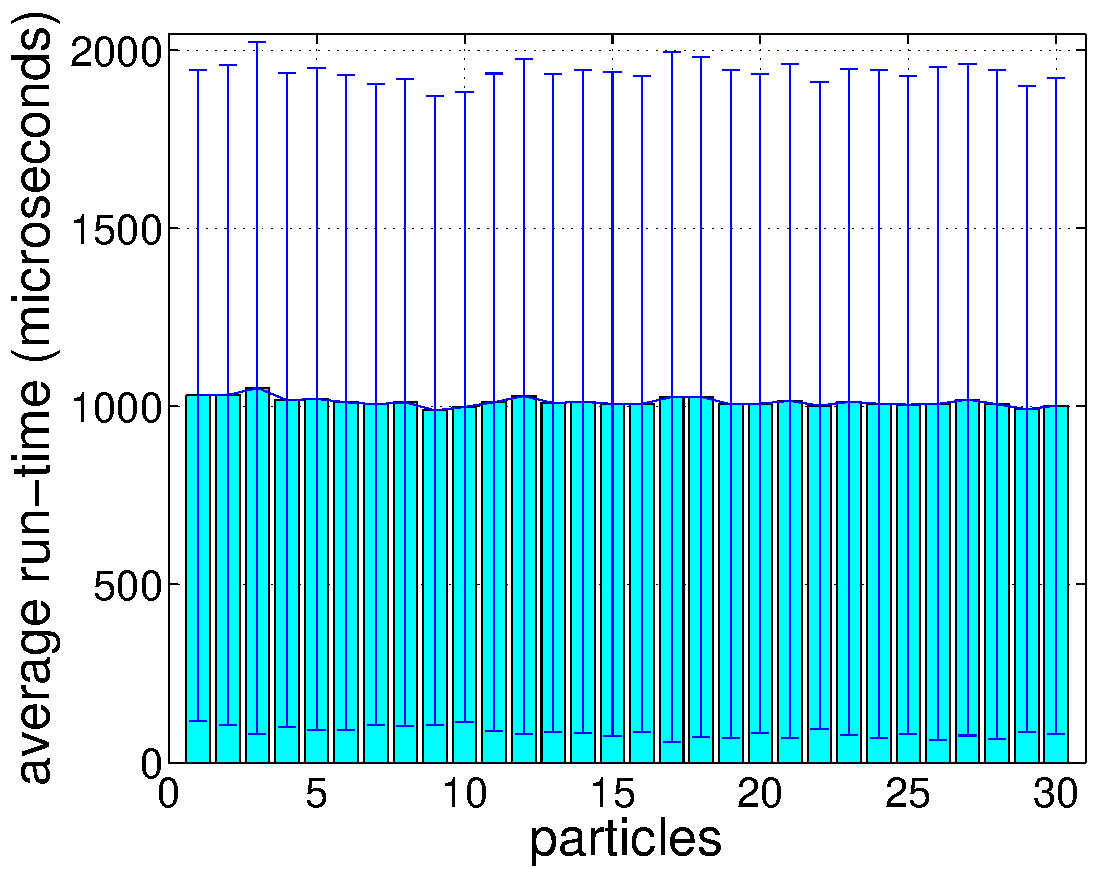
\includegraphics[width=0.31\columnwidth,keepaspectratio]{../Thesis/graphs/graph_particle_times_mit-csail-3rd-floor-2005-12-17-run4.pdf}
 }
 \subfigure[] {
 \centering
 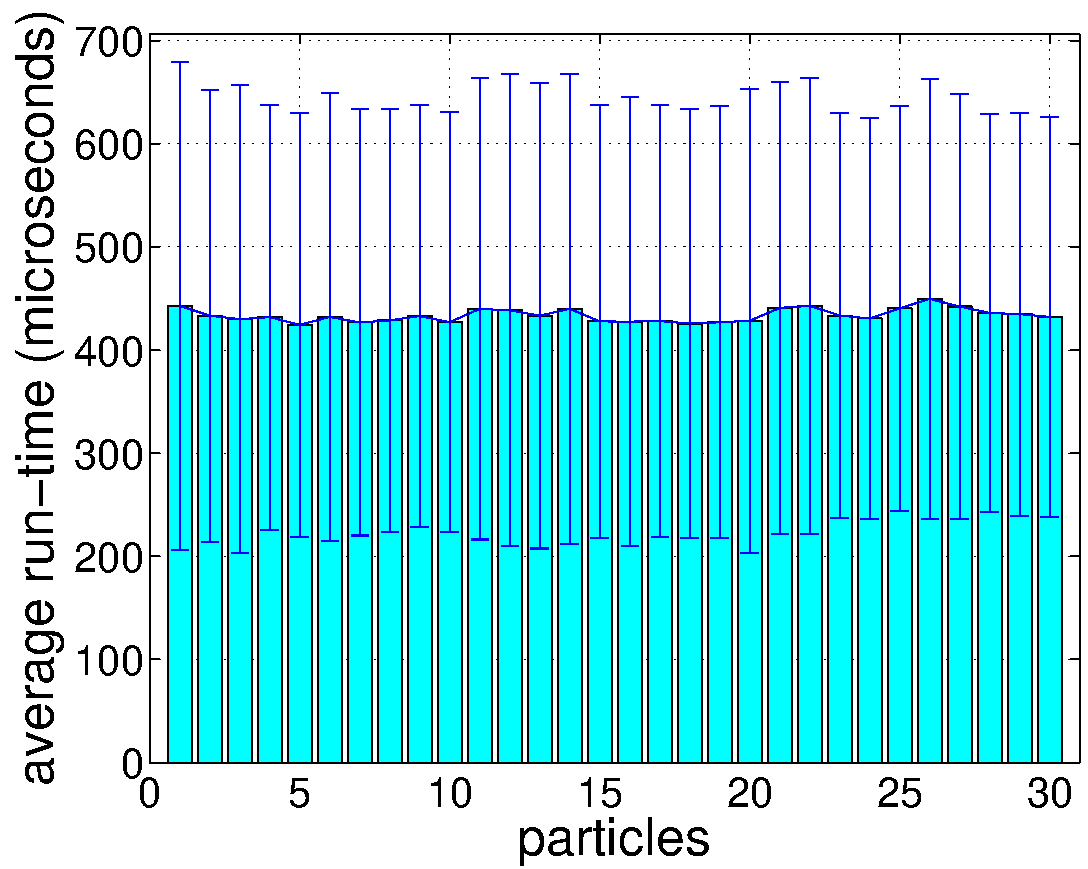
\includegraphics[width=0.31\columnwidth,keepaspectratio]{../Thesis/graphs/graph_particle_times_edmonton_3.pdf}
 }
\end{figure}
}
\end{frame}

\begin{frame}
\frametitle{\FFD Performance According to Number of Particles}
\only<1>{
\begin{itemize}
  %\item \FFD has to persistently run in the background
  %\item Particle-filter systems: each particle has its own instance of \FFD
  %\item Hence, the overall run-time is increased \pause
  \item Investigate how number of particles affects on \FFD performance 
  \item We change the number of particles in different maps
  \item Measure how overall run-time is increased
  %\item Each bar represents a run with a specific number of particles
  %\item Vertical axis: mean run-time of \FFD for the configuration
  %\item Error-bars: standard deviation of each configuration run-time
\end{itemize}
}
\only<2>{
\setcounter{subfigure}{0}
\begin{figure}
 \centering 
 \subfigure[] {
 \centering
 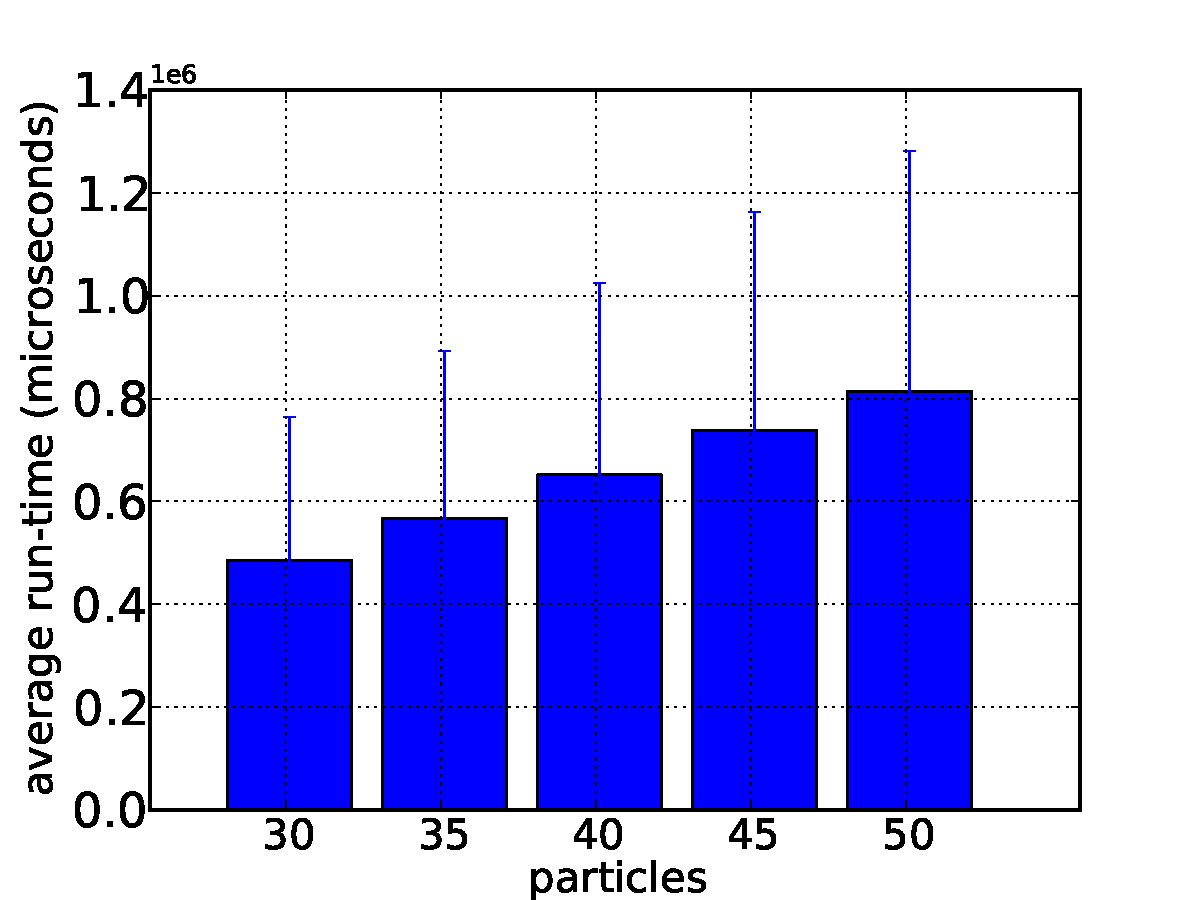
\includegraphics[width=0.31\columnwidth,keepaspectratio]{../Thesis/graphs/plot_ubremen-cartesium-demo2_gfs_log_Particles.pdf}
 }
 \subfigure[] {
 \centering
 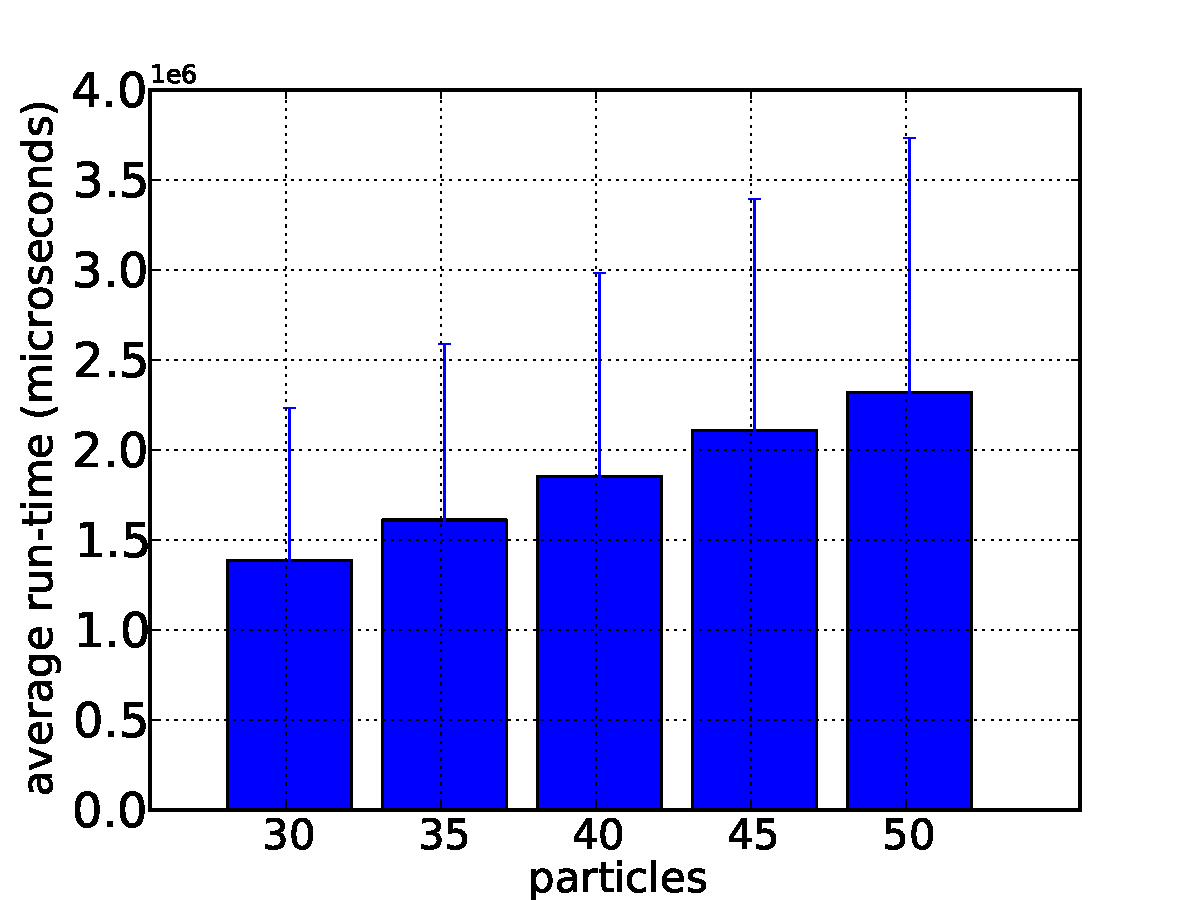
\includegraphics[width=0.31\columnwidth,keepaspectratio]{../Thesis/graphs/plot_fr079-sm_log_Particles.pdf}
 }
 \subfigure[] {
 \centering
 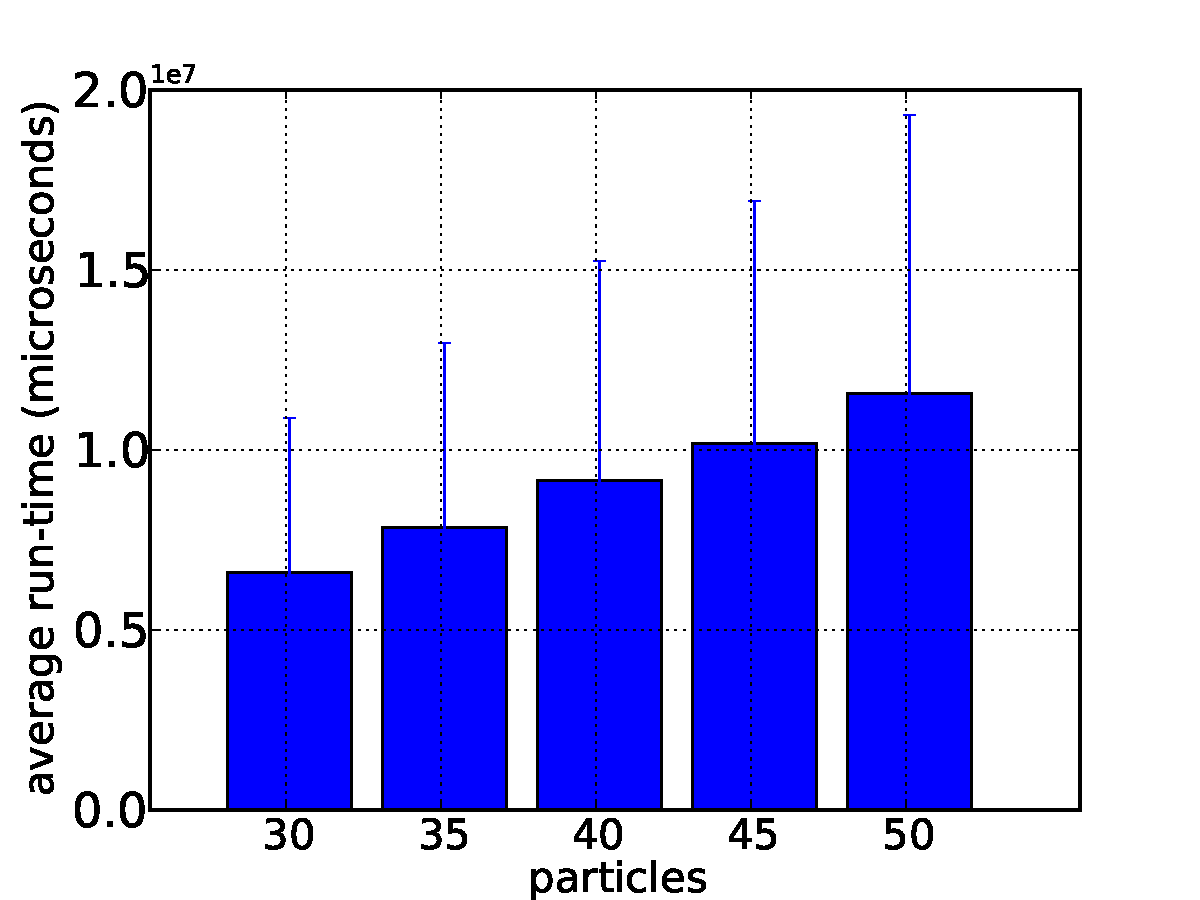
\includegraphics[width=0.31\columnwidth,keepaspectratio]{../Thesis/graphs/plot_fr-campus-20040714_carmen_log_Particles.pdf}
 }
 \subfigure[] {
 \centering
 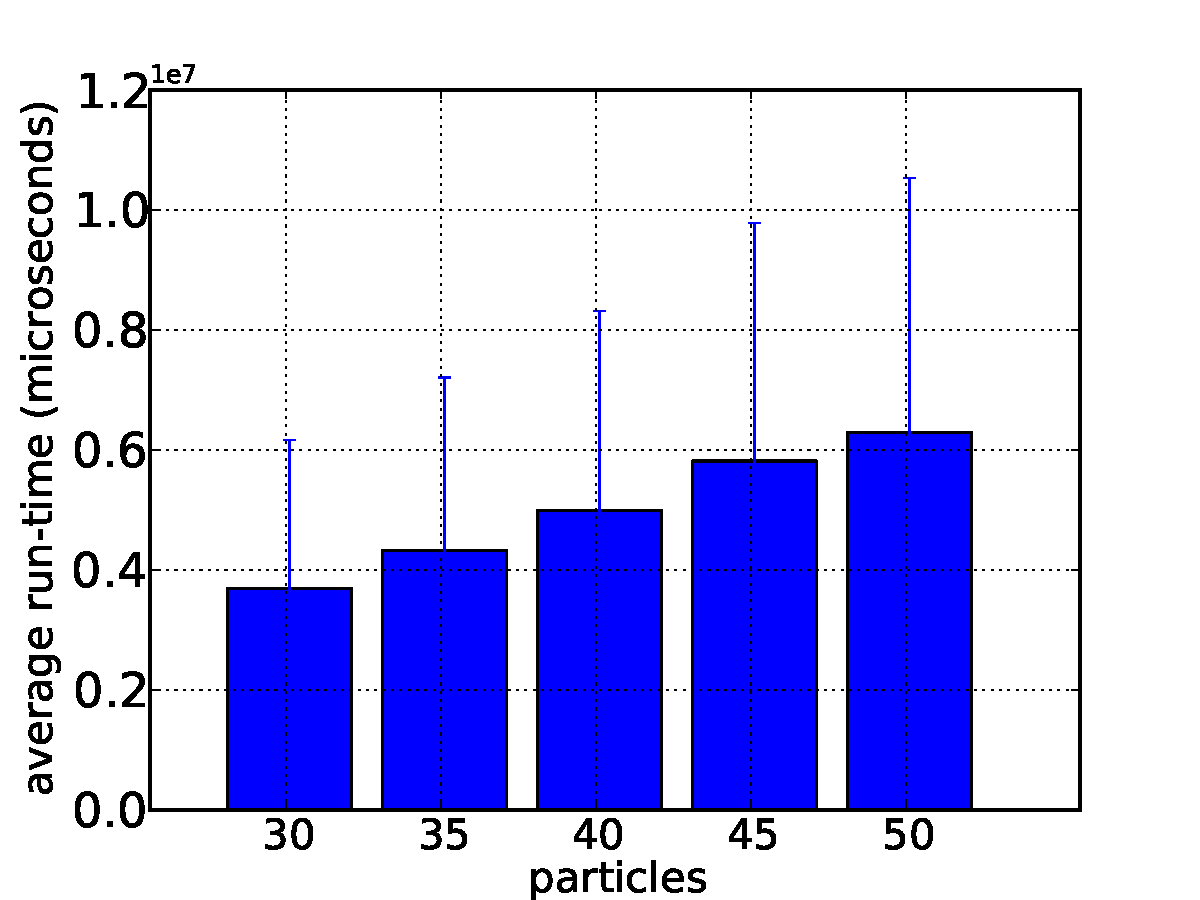
\includegraphics[width=0.31\columnwidth,keepaspectratio]{../Thesis/graphs/plot_mit-csail-3rd-floor-2005-12-17-run4_flaser_log_Particles.pdf}
 }
 \subfigure[] {
 \centering
 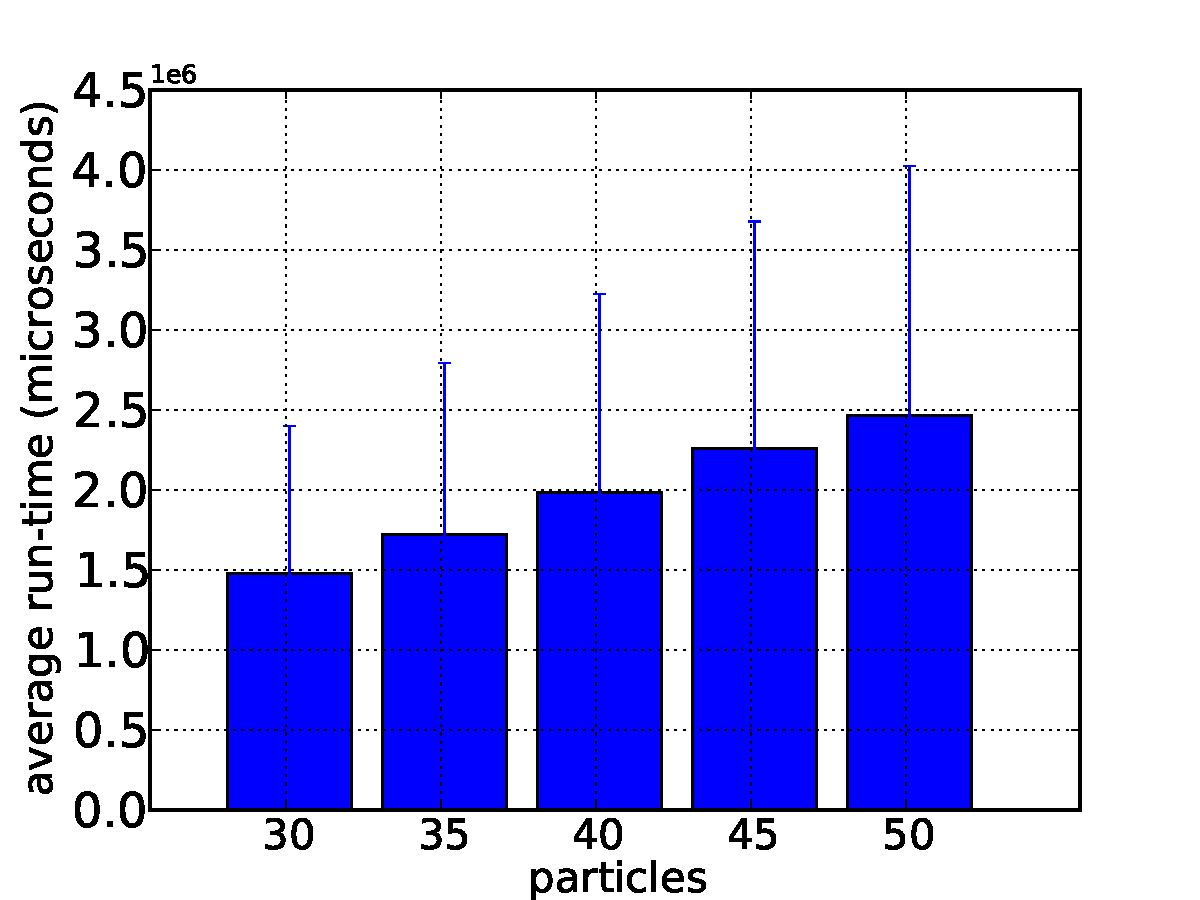
\includegraphics[width=0.31\columnwidth,keepaspectratio]{../Thesis/graphs/plot_edmonton_3_log_Particles.pdf}
 }
\end{figure}
}
\end{frame}

% \begin{frame}
% \frametitle{Results}
% \begin{itemize}
%   \item Each group of bars represents run in a specific environment 
%   \item Y axis measures the average execution time (microseconds)
%   	\begin{itemize}
%   	  \item on a \emph{logaritmic scale}
%     \end{itemize} 
%   \item \WFD is faster than \SOTA by two orders of magnitude 
%   \item \FFD is faster than \WFD by an order of magnitude 
% \end{itemize}
% \end{frame}